% Provenance (never printed): old terminale S material on magmatism in
% subduction zones (volcanic arcs above the slab, water released by the slab
% and hydrous melting of the mantle wedge, andesitic volcanism and granitoid
% plutons, growth of the continental crust). Owner (Sync 0): volcanic arc,
% hydrous melting, granodiorite, batholith, continental growth. Subduction,
% slab, Wadati-Benioff zone, blueschist and eclogite are g11.06's; partial and
% decompression melting and peridotite g11.05's; andesite, diorite, rhyolite,
% pluton g11.08's; continental crust g12.01's; magma, explosive eruption Book 1's
% (g7): recalled, never redefined. Figures: figdata/grade-12/arc_magmatism.py
% (GVP volcanoes, ComCat NE Japan band, dry solidus via grade-11
% geotherm_solidus.py, wet solidus brackets of Wang 2020 and Kawamoto-Holloway 1997).
\chapter{O magmatismo das zonas de subducção}\label{ch:g12:subduction-magmatism}

Em 18 de maio de 1980, às 8h32 da manhã, um terremoto de magnitude 5.1
sacudiu o monte Santa Helena. No mesmo instante, o flanco norte do vulcão,
que vinha se estufando para fora cerca de dois metros por dia, deslizou: a
maior avalanche de detritos da história registrada, cerca de
\qty{2.5}{km^3} de rocha. Livre da sua carga, o magma rico em gás do
interior explodiu de lado através da cicatriz, a nada menos que
\qty{480}{km/h}, derrubando florestas em \qty{600}{km^2}. Em quinze
minutos, uma coluna de cinzas se erguia a mais de \qty{24}{km} de altura, e
a erupção continuou por nove horas. Sessenta e uma pessoas morreram ou
nunca foram encontradas.
% ledger: usgs:b2-msh-1980, usgs:msh-deaths

\begin{omfigure}
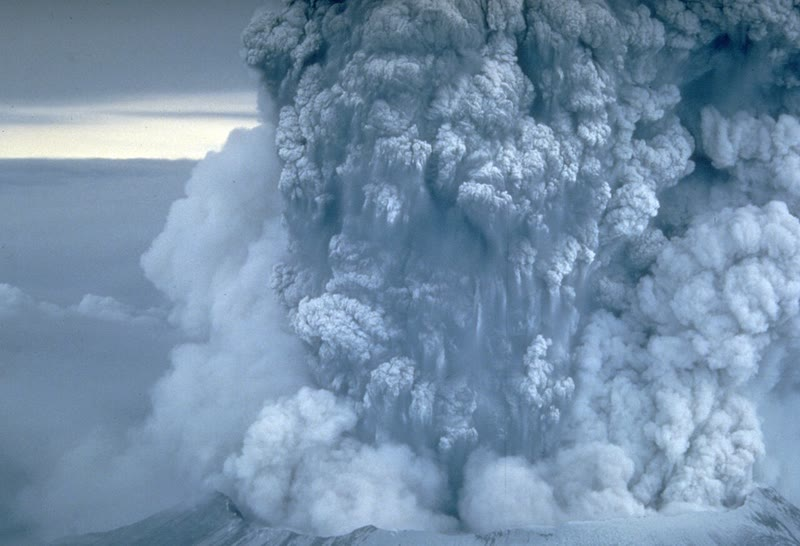
\includegraphics[width=0.55\linewidth]{images/book2/g12-swanson-st-helens-plume.jpg}

{\small A coluna de cinzas do monte Santa Helena em 18 de maio de 1980, que
subiu a mais de \qty{24}{km} em menos de quinze minutos. Fotografia Donald
A.~Swanson, USGS (domínio público).}
\end{omfigure}
% ledger: photo:g12-st-helens, usgs:b2-msh-1980

O monte Santa Helena é um de uma fileira de vulcões --- Baker, Rainier,
Hood, Shasta e outros --- que fica acima do lugar onde uma pequena placa
oceânica, a placa Juan de Fuca, afunda sob a América do Norte. Este capítulo
pergunta por que se encontram vulcões ali, por que as suas erupções são tão
muitas vezes violentas, e o que acontece com o magma que nunca chega à
superfície.
% ledger: earle:cascades

\begin{recall}
Numa \omterm{def:g11:subduction-zones:subduction}{zona de subducção}, uma placa de \omterm{def:g11:ocean-ridges:oceanic-lithosphere}{litosfera oceânica} volta a afundar no
manto sob outra placa; os seus terremotos, a \omterm{def:g11:subduction-zones:benioff}{zona de Wadati--Benioff}, seguem
a \omterm{def:g11:subduction-zones:slab}{laje} até \qty{670}{km} de profundidade (\cref{ch:g11:subduction-zones}). O
manto é feito de \omterm{def:g11:ocean-ridges:peridotite}{peridotito}; ele é sólido, mas uma rocha que sobe e fica
menos comprimida pode se fundir em parte, por \omterm{def:g11:ocean-ridges:partial-melting}{fusão por descompressão}, como
sob uma dorsal (\cref{ch:g11:ocean-ridges}). O \omterm{def:g11:igneous-rocks:rock-names}{andesito} é uma \omterm{def:g11:igneous-rocks:volcanic-plutonic}{rocha
vulcânica} \omterm{def:g11:igneous-rocks:felsic-mafic}{intermediária} entre o basalto e o \omterm{def:g11:igneous-rocks:rock-names}{riolito}, o \omterm{def:g11:igneous-rocks:rock-names}{diorito} é o seu
equivalente plutônico, e um \omterm{def:g11:igneous-rocks:intrusion}{plúton} é um grande corpo de magma que esfriou
no subsolo (\cref{ch:g11:igneous-rocks}). A \omterm{def:g12:continental-crust:continental-crust}{crosta continental} é espessa e
leve, feita principalmente de rocha granítica em cima
(\cref{ch:g12:continental-crust}). Uma erupção explosiva despedaça o magma
com o seu próprio gás (Livro 1, 7º ano).
\end{recall}
% ledger: tulane:magma-types, tulane:intrusions, rg14:crust

\section{Os arcos vulcânicos}

A maioria dos vulcões ativos em terra não fica em lugares quaisquer. Dos
1214 vulcões que entraram em erupção desde o fim da última era glacial e
estão listados no catálogo do Global Volcanism Program, 838 --- mais de dois
em cada três --- ficam acima de uma \omterm{def:g11:subduction-zones:subduction}{zona de subducção}. Em volta do Pacífico,
eles formam um anel quase contínuo, muitas vezes chamado de Anel de Fogo, e
cada fileira deles corre paralela a uma fossa, do lado da placa que não
afunda.
% values: n_volcanoes 1214, n_subduction 838, frac_subduction 0.690 (arc_magmatism.py)
% ledger: data:gvp, tulane:arc

\begin{omfigure}
\begin{tikzpicture}
\begin{axis}[ommap, width=\linewidth, xtick={-180,-90,...,180}, ytick={-60,0,60},
  legend style={font=\scriptsize, at={(0.5,-0.13)}, anchor=north, legend columns=3,
    /tikz/every even column/.append style={column sep=6pt}}]
\addplot[fill=omLithAlluv, draw=black!45, line width=0.2pt, forget plot] table {figdata/out/shared-geo-land.dat};
\addplot[black!70, line width=0.5pt, forget plot] table {figdata/out/shared-geo-school-subduction.dat};
\addplot[fill=black!70, draw=none, forget plot] table {figdata/out/shared-geo-school-teeth.dat};
% computed in figdata/grade-12/arc_magmatism.py; ledger: data:gvp, data:pb2002, data:ne-land
\addplot[only marks, mark=triangle*, mark size=1.1pt, black!40] table[x=lon, y=lat] {figdata/out/grade-12-arc_magmatism-world-other.dat};
\addplot[only marks, mark=triangle*, mark size=1.3pt, omThm] table[x=lon, y=lat] {figdata/out/grade-12-arc_magmatism-world-sub.dat};
\addlegendimage{black!70, line width=0.5pt}
\legend{{outros vulcões}, {vulcões acima de uma zona de subducção}, {fossa}}
\end{axis}
\end{tikzpicture}

{\small Os vulcões ativos desde o fim da última era glacial, em vermelho
quando ficam acima de uma \omterm{def:g11:subduction-zones:subduction}{zona de subducção}, com as fossas (linha preta,
triângulos do lado da placa que se sobrepõe). Dados: Global Volcanism
Program do Smithsonian; limites de placas de Bird (2003); terras emersas do
Natural Earth.}
\end{omfigure}
% values: n_subduction 838 of 1214 (arc_magmatism.py)

\begin{definition}[Arco vulcânico]\label{def:g12:subduction-magmatism:arc}
Um \emph{arco vulcânico}\index{arco vulcanico@arco vulcânico} é uma fileira
de vulcões na placa que se sobrepõe de uma \omterm{def:g11:subduction-zones:subduction}{zona de subducção}, paralela à
fossa, acima do lugar onde a \omterm{def:g11:subduction-zones:slab}{laje} atingiu uma profundidade de cerca de cem
quilômetros. É um \emph{arco insular} quando se ergue do fundo do mar, como
no Japão ou na Indonésia, e um arco continental quando fica sobre um
continente, como nos Andes ou nas Cascatas.
\end{definition}
% ledger: tulane:arc, earle:arc-water, earle:cascades, sa06:slab-depth

A borda do arco mais próxima da fossa se chama \textbf{frente vulcânica}: do
lado da fossa, não há nenhum vulcão. A que profundidade fica a \omterm{def:g11:subduction-zones:slab}{laje} abaixo
dela?

\begin{proposition}[A laje sob a frente vulcânica]\label{prop:g12:subduction-magmatism:depth}
Se a \omterm{def:g11:subduction-zones:slab}{laje} é um plano que mergulha com um ângulo $\theta$ a partir da fossa,
e se a frente vulcânica fica a uma distância horizontal $d$ da fossa, então
o topo da \omterm{def:g11:subduction-zones:slab}{laje} fica sob a frente a uma profundidade
\[
  H = d \tan\theta .
\]
\end{proposition}

\begin{proof}
Tome um corte vertical através da fossa. A \omterm{def:g11:subduction-zones:slab}{laje}, a superfície e a vertical
sob a frente formam um triângulo retângulo, com o ângulo reto sob a frente:
o lado ao longo da superfície é $d$, o lado vertical é $H$, e o ângulo na
fossa é $\theta$. Logo $\tan\theta = H/d$.
\end{proof}

Uma compilação de 839 centros vulcânicos ao longo de \qty{33000}{km} de
arcos mediu $H$ sob cada um deles: em média sobre trechos de arco de
\qty{500}{km}, ela vai de 72 a \qty{173}{km}, com uma média de
\qty{105}{km}. Os arcos acima de \omterm{def:g11:subduction-zones:slab}{lajes} íngremes ficam perto da sua fossa,
os arcos acima de \omterm{def:g11:subduction-zones:slab}{lajes} de mergulho suave ficam longe dela, mas a \omterm{def:g11:subduction-zones:slab}{laje} sob
eles está sempre a cerca de cem quilômetros de profundidade.
% ledger: sa06:slab-depth

\begin{method}[Encontrar a laje sob um vulcão]\label{met:g12:subduction-magmatism:slab}
\begin{enumerate}
  \item Tome os terremotos de uma faixa estreita através do arco, e
        represente a sua profundidade em função da sua distância através
        dele, em escala verdadeira.
  \item Guarde os terremotos com mais de cerca de \qty{70}{km} de
        profundidade: os mais rasos também ocorrem na placa que se sobrepõe e
        na falha entre as duas placas.
  \item Trace a reta, ou leia a profundidade, dos terremotos profundos sob a
        frente vulcânica: é a profundidade da \omterm{def:g11:subduction-zones:slab}{laje} ali.
  \item Verifique-a com $H = d\tan\theta$, medindo $d$ a partir da fossa e
        o mergulho $\theta$ no corte.
\end{enumerate}
\end{method}

\begin{omfigure}
\begin{tikzpicture}
\begin{axis}[omsection, name=jp, scale only axis, width=0.8\linewidth, height=0.2857\linewidth,
  xmin=0, xmax=700, ymin=0, ymax=250, y dir=reverse,
  xlabel={distância a leste de \ang{138}~L (\unit{km})}, ylabel={profundidade (\unit{km})},
  xtick={0,100,...,700}, ytick={0,50,...,250}, tick label style={font=\small},
  every axis label/.append style={font=\small}]
% computed in figdata/grade-12/arc_magmatism.py; ledger: data:b2-usgs-ne-japan, data:gvp, data:pb2002
\addplot[only marks, mark=*, mark size=0.55pt, black!35] table[x=x_km, y=depth] {figdata/out/grade-12-arc_magmatism-jp-quakes.dat};
\addplot[omDef, line width=0.9pt, dashed] table[x=x_km, y=depth] {figdata/out/grade-12-arc_magmatism-jp-slab.dat};
\addplot[only marks, mark=triangle*, mark size=2.6pt, omThm] table[x=x_km, y expr=-7] {figdata/out/grade-12-arc_magmatism-jp-volc.dat};
\draw[omThm, densely dotted, line width=0.8pt] (axis cs:259.2,0) -- (axis cs:259.2,98.2);
\fill[omThm] (axis cs:259.2,98.2) circle (1.6pt);
\coordinate (front) at (axis cs:259.2,-14);
\coordinate (trench) at (axis cs:528.9,-14);
\coordinate (H) at (axis cs:262,60);
\coordinate (slab) at (axis cs:95,228);
\draw[black, line width=0.9pt] (axis cs:528.9,-12) -- (axis cs:528.9,0);
\end{axis}
\node[font=\scriptsize, anchor=south, text=omThm] at (front) {frente vulcânica (Iwate)};
\node[font=\scriptsize, anchor=south] at (trench) {Fossa do Japão};
\node[font=\scriptsize, anchor=west, text=omThm, fill=white, inner sep=1pt] at (H) {\qty{98}{km}};
\node[font=\scriptsize, anchor=west, text=omDef, fill=white, inner sep=1pt] at (slab) {laje, com mergulho de cerca de \ang{20}};
\end{tikzpicture}

{\small Um corte através do nordeste do Japão em escala verdadeira: os
terremotos de magnitude 4.5 ou mais entre \ang{37.5} e \ang{40.5}~Norte,
1976--2025 (em cinza), os vulcões da mesma faixa (triângulos vermelhos) e a
reta ajustada aos terremotos com mais de \qty{70}{km} de profundidade (em
azul, tracejada). Dois em cada cinco dos eventos rasos a leste de
\ang{141.5}~Leste datam de 2011, o ano do grande terremoto de março. Dados:
catálogo de terremotos do USGS; Global Volcanism Program do Smithsonian;
limites de placas de Bird (2003).}
\end{omfigure}
% values: shallow (<70 km) events east of 141.5 E: 3622, of which 1451 in 2011 (0.40); ledger usgs:tohoku
% values: jp_front_lon 141.0 (x 259.2 km), jp_trench_lon 144.12 (x 528.9), jp_front_trench_km 269.4, jp_dip_deg 19.98, jp_H_geom 98.0, bin_141_median 98.15, jp_slab_depth_front 105.6 (arc_magmatism.py)

\begin{example}[O nordeste do Japão]\label{ex:g12:subduction-magmatism:japan}
Na faixa da figura, o vulcão mais a leste é o Iwate, a \ang{141.0}~Leste, e
a Fossa do Japão fica a \ang{144.1}~Leste. Um grau de longitude ali vale
$111.2\cos\ang{39} \approx \qty{86.4}{km}$, logo $d \approx 3.12 \times 86.4
\approx \qty{270}{km}$. Os terremotos profundos mergulham cerca de \ang{20},
e
\[
  H = 270 \times \tan\ang{20} \approx \qty{98}{km}.
\]
Os terremotos com mais de \qty{70}{km} de profundidade que ficam sob a
própria frente têm uma profundidade mediana de \qty{98}{km}: os dois
concordam, perto da média mundial.
\end{example}
% values: km_per_deg_lon 86.415, jp_front_trench_km 269.4, jp_dip_deg 19.98, jp_H_geom 97.98, bin_141_median 98.15 (arc_magmatism.py)

\section{A água funde o manto}

Sob um arco, a \omterm{def:g11:subduction-zones:slab}{laje} é fria, e a \omterm{def:g11:ocean-ridges:oceanic-lithosphere}{crosta oceânica} em cima dela também: ela não
pode se fundir. O magma precisa vir do manto quente acima da \omterm{def:g11:subduction-zones:slab}{laje}, a
\textbf{cunha do manto}. Mas a cunha não está subindo, então ela não pode se
fundir por descompressão como sob uma dorsal. Outra coisa abaixa a sua
temperatura de fusão: a água.
% ledger: earle:settings (subducted crust stays cool), earle:flux-melting, earle:arc-water

A \omterm{def:g11:ocean-ridges:oceanic-lithosphere}{crosta oceânica} é encharcada de água do mar perto da dorsal onde se forma,
e grande parte dessa água acaba presa dentro dos seus minerais, sobretudo na
serpentina, formada a partir da olivina e do piroxênio da crosta. À medida
que a \omterm{def:g11:subduction-zones:slab}{laje} afunda e se aquece, esses minerais se decompõem e liberam a sua
água. A água sobe para o \omterm{def:g11:ocean-ridges:peridotite}{peridotito} quente da cunha acima.
% ledger: earle:arc-water, tulane:arc

\begin{definition}[Fusão hidratada]\label{def:g12:subduction-magmatism:hydrous-melting}
A \emph{fusão hidratada}\index{fusao hidratada@fusão hidratada} (ou fusão por fluxo) é a
\omterm{def:g11:ocean-ridges:partial-melting}{fusão parcial} de uma rocha causada pela adição de água, que abaixa a
temperatura em que a rocha começa a se fundir.
\end{definition}
% ledger: earle:flux-melting, earle:arc-water

A temperatura em que uma rocha começa a se fundir, a uma dada pressão, é o
seu \textbf{solidus}. Para o \omterm{def:g11:ocean-ridges:peridotite}{peridotito} seco, ele é bem conhecido; com água,
é muito mais difícil de medir, e os valores publicados ainda diferem de 200
a \qty{600}{\celsius}. Os experimentos mais recentes o situam entre 950 e
\qty{1000}{\celsius} a \qty{3}{GPa}, cerca de \qty{95}{km} de profundidade,
e um pouco acima de \qty{1000}{\celsius} de 5 a \qty{11}{GPa}. O \omterm{def:g11:ocean-ridges:peridotite}{peridotito}
seco a \qty{3}{GPa} só começa a se fundir a cerca de \qty{1470}{\celsius}:
a água abaixa o solidus em cerca de \qty{500}{\celsius}.
% values: dry_T_3gpa 1473.4, dry_minus_wet_3gpa 498, z_3gpa_km 95.2, dry_minus_wet_5gpa 658 (arc_magmatism.py)
% ledger: hirschmann:solidus, wang20:wet-solidus, kh97:wet-solidus, data:prem, earth:gmean

\begin{omfigure}
\begin{tikzpicture}
\begin{axis}[omrecord, name=sol, scale only axis, width=0.62\linewidth, height=6.2cm,
  xmin=700, xmax=1900, ymin=0, ymax=230, y dir=reverse,
  xlabel={temperatura (\unit{\celsius})}, ylabel={profundidade (\unit{km})},
  xtick={800,1000,...,1800}, ytick={0,50,...,200}, axis y line*=left]
% computed in figdata/grade-12/arc_magmatism.py (dry: Hirschmann 2000 with PREM pressures; wet: Wang 2020, Kawamoto-Holloway 1997)
\addplot[omProp, line width=1.2pt] table[x=T_dry, y=depth_km] {figdata/out/grade-12-arc_magmatism-solidus.dat};
\addplot[omDef, line width=2.4pt] coordinates {(950,95.24) (1000,95.24)};
\addplot[omDef, line width=1.2pt] coordinates {(1000,155.6) (1000,216.3)};
\draw[-{Stealth}, black!70, line width=0.8pt] (axis cs:1460,95.24) -- (axis cs:1015,95.24);
\coordinate (gap) at (axis cs:1240,95.24);
\coordinate (dry) at (axis cs:1600,40);
\coordinate (wet) at (axis cs:1015,190);
\coordinate (wet3) at (axis cs:975,90);
\end{axis}
\begin{axis}[scale only axis, width=0.62\linewidth, height=6.2cm, at={(sol.south west)}, anchor=south west,
  xmin=700, xmax=1900, ymin=0, ymax=230, y dir=reverse, axis x line=none, axis y line*=right,
  axis line style={-}, ylabel={pressão (\unit{GPa})},
  ytick={34.9,65.1,95.2,125.5,155.6,185.9,216.3}, yticklabels={1,2,3,4,5,6,7},
  every axis label/.append style={font=\small}, tick label style={font=\small}]
% pressure ticks at the PREM depths of 1-7 GPa (arc_magmatism.depth_at_pressure)
\end{axis}
\node[font=\scriptsize, anchor=south] at ([yshift=2pt]gap) {cerca de \qty{500}{\celsius}};
\node[font=\scriptsize, text=omProp, anchor=west, align=left] at (dry) {o peridotito seco\\começa a se fundir};
\node[font=\scriptsize, text=omDef, anchor=west, align=left] at (wet) {com água: um pouco\\acima de \qty{1000}{\celsius}};
\node[font=\scriptsize, text=omDef, anchor=south] at ([yshift=2pt]wet3) {950--1000};
\end{tikzpicture}

{\small A temperatura em que o \omterm{def:g11:ocean-ridges:peridotite}{peridotito} do manto começa a se fundir, em
função da profundidade: seco (em laranja) e saturado de água (em azul, as
duas faixas medidas até agora). À profundidade da \omterm{def:g11:subduction-zones:slab}{laje} sob os arcos, cerca
de \qty{100}{km}, a água a abaixa em cerca de \qty{500}{\celsius}. Fontes:
Hirschmann (2000), com as densidades do PREM; Wang e colaboradores (2020);
Kawamoto e Holloway (1997).}
\end{omfigure}
% values: dry_T_3gpa 1473.4, dry_T_100km 1489.4, P_100km_gpa 3.157 (arc_magmatism.py)

Assim, a água faz o que o aquecimento sozinho não conseguiria: ela faz uma
parte da cunha quente se fundir. O magma, mais leve que o manto sólido em
volta, sobe em direção à superfície; uma parte entra em erupção, muito mais
fica e esfria no subsolo. O lugar onde a água é liberada, e onde a cunha
acima dela é quente o bastante para se fundir uma vez molhada, é o que fixa
a frente vulcânica a cerca de cem quilômetros acima da \omterm{def:g11:subduction-zones:slab}{laje}.
% ledger: earle:arc-water, tulane:arc, sa06:slab-depth, wang20:wet-solidus (position of the volcanic front controlled by melting in the wedge)

\begin{omfigure}
\begin{tikzpicture}[x=1cm, y=1cm, font=\scriptsize]
  % mantle
  \fill[omLithPeridotite!45] (0,-0.9) -- (7.4,-0.9) -- (7.5,-0.85) -- (6.5,-1.6) -- (5.5,-2.6) -- (4.5,-3.8)
    -- (4.25,-4.3) -- (0,-4.3) -- cycle;
  % sea and overriding continental crust
  \fill[omSea] (8.0,0) -- (12,0) -- (12,-0.4) -- (8.5,-0.4) -- cycle;
  \fill[omLithGranite!55] (0,0.1) -- (8.0,0.1) -- (8.5,-0.4) -- (7.5,-0.85) -- (7.4,-0.9) -- (0,-0.9) -- cycle;
  % the slab
  \fill[omLithBasalt!45, draw=black!60] (12,-0.4) -- (8.5,-0.4) -- (7.5,-0.85) -- (6.5,-1.6) -- (5.5,-2.6) -- (4.5,-3.8)
    -- (4.25,-4.3) -- (5.15,-4.3) -- (5.2,-4.3) -- (6.15,-3.15) -- (7.1,-2.2) -- (8.0,-1.55) -- (8.9,-1.2) -- (12,-1.2) -- cycle;
  \node at (10.4,-0.8) {litosfera oceânica};
  \node[anchor=west] at (6.0,-3.4) {laje que afunda};
  % melting in the wedge, rising magma, plutons, volcano
  \fill[omThm!35, draw=omThm, densely dashed] (5.2,-1.75) ellipse (0.6 and 0.3);
  \node[omThm] at (5.2,-1.75) {fusão};
  \foreach \y in {-1.3,-1.05} \fill[omThm!80] (5.2,\y) circle (0.07);
  \fill[omLithGranite, draw=black!60] (4.75,-0.55) ellipse (0.42 and 0.2);
  \fill[omLithGranite, draw=black!60] (5.65,-0.4) ellipse (0.32 and 0.16);
  \node[anchor=east] at (4.25,-0.55) {plútons};
  \draw[omThm, line width=1pt] (5.2,0.1) -- (5.2,-0.85);
  \fill[black!65] (4.75,0.1) -- (5.2,0.75) -- (5.65,0.1) -- cycle;
  \node[anchor=south] at (5.2,0.8) {vulcão};
  % water released by the slab
  \foreach \x/\y in {6.5/-1.6, 6.0/-2.1, 5.6/-2.5}
    \draw[omDef, -{Stealth}, line width=0.7pt, decorate, decoration={snake, amplitude=0.6pt, segment length=4pt, post length=1.5mm}]
      (\x,\y) -- ++(-0.3,0.3);
  \draw[omDef, line width=0.3pt] (7.5,-2.75) -- (6.35,-2.0);
  \node[omDef, anchor=west, align=left] at (7.5,-2.75) {água liberada\\pela laje};
  % labels and depth scale
  \node at (1.8,-0.4) {crosta continental};
  \node[black!70, align=center] at (2.3,-3.6) {cunha do manto quente\\(peridotito)};
  \node[anchor=south] at (8.5,0.12) {fossa};
  \draw[black!60, |-|] (0.4,0.1) -- node[left, align=right] {cerca de\\\qty{100}{km}} (0.4,-2.96);
  \draw[black!45, densely dotted] (0.4,-2.96) -- (5.2,-2.96);
  \fill[black!70] (5.2,-2.96) circle (1.3pt);
  \draw[black!45, densely dotted] (5.2,-2.96) -- (5.2,-2.05);
\end{tikzpicture}

{\small O magmatismo numa \omterm{def:g11:subduction-zones:subduction}{zona de subducção} (esquemático, fora de escala).
À medida que a \omterm{def:g11:subduction-zones:slab}{laje} se aquece, os seus minerais liberam a sua água, que sobe
para a cunha do manto quente e a faz se fundir em parte. O magma sobe: uma
parte entra em erupção nos vulcões, uma parte maior esfria na crosta como
\omterm{def:g11:igneous-rocks:intrusion}{plútons}.}
\end{omfigure}
% ledger: earle:arc-water, earle:flux-melting, tulane:arc, tulane:ridge-rocks, sa06:slab-depth

\section{Andesitos e granodioritos}

Os primeiros líquidos do \omterm{def:g11:ocean-ridges:peridotite}{peridotito} úmido não são basálticos. Em
experimentos a \qty{1}{GPa}, o \omterm{def:g11:ocean-ridges:peridotite}{peridotito} saturado de água dá líquidos de
composição andesítica. Ao subir através da crosta espessa do arco, os magmas
também mudam à medida que esfriam, de basálticos para andesíticos e
riolíticos. Os magmas de arco são, portanto, mais ricos em sílica que os
basaltos das dorsais --- o magma andesítico contém de 55 a
\qty{65}{\percent} dela ---, e carregam a água que os formou.
% ledger: kh97:wet-solidus (andesitic melts at 1 GPa), tulane:eruptions, tulane:ridge-rocks, tulane:magma-types

As duas propriedades tornam as suas erupções violentas. Quanto mais sílica
um magma contém, mais viscoso ele é, e mais difícil é para o seu gás
escapar; as erupções explosivas são favorecidas por um alto teor de gás e
uma alta viscosidade, como nos magmas andesíticos e riolíticos. Quase todos
os vulcões compostos ficam acima de \omterm{def:g11:subduction-zones:subduction}{zonas de subducção}: cones de milhares de
metros de altura e de até \qty{20}{km} de largura, com encostas de 10 a 30
graus, cujas erupções vão de tranquilos derrames de lava a explosões. Sob o
monte Santa Helena, uma câmara magmática de cerca de \qty{1}{km} de largura
se estende de cerca de 6 a \qty{14}{km} de profundidade.
% ledger: tulane:magma-types, tulane:eruptions, earle:composite

A maior parte do magma de arco nunca entra em erupção. Ele esfria lentamente
na crosta e se cristaliza em rochas de grãos grossos.

\begin{definition}[Granodiorito]\label{def:g12:subduction-magmatism:granodiorite}
O \emph{granodiorito}\index{granodiorito} é uma \omterm{def:g11:igneous-rocks:volcanic-plutonic}{rocha plutônica} de grãos
grossos semelhante ao granito, mas com mais plagioclásio que feldspato
potássico: de 20 a \qty{60}{\percent} dos seus minerais claros são quartzo,
e de 65 a \qty{90}{\percent} do seu feldspato é plagioclásio; ele contém
muitas vezes biotita ou hornblenda.
\end{definition}
% ledger: bgs:granodiorite

\begin{omfigure}
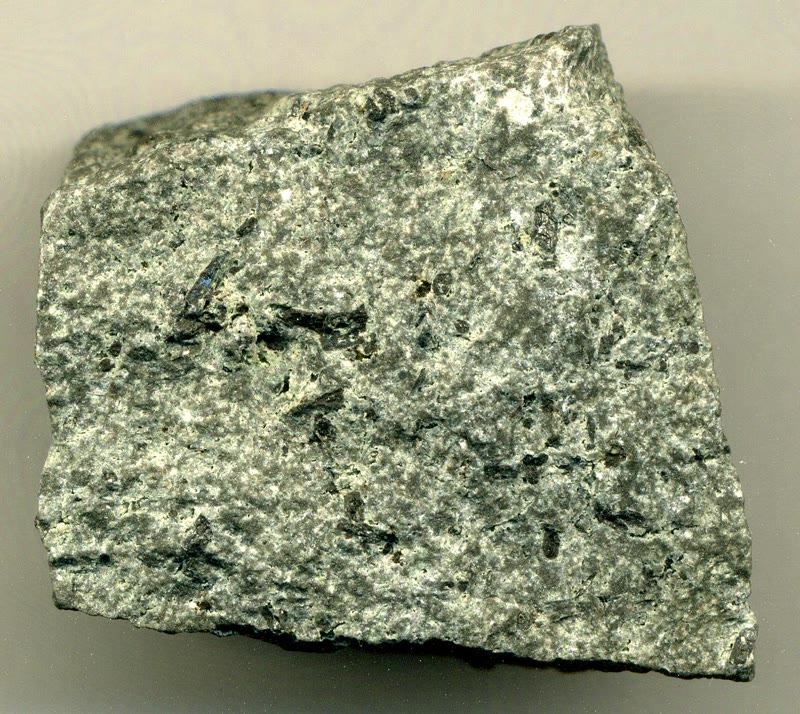
\includegraphics[height=4.4cm]{images/book2/g12-stjohn-andesite.jpg}\hspace{0.03\linewidth}%
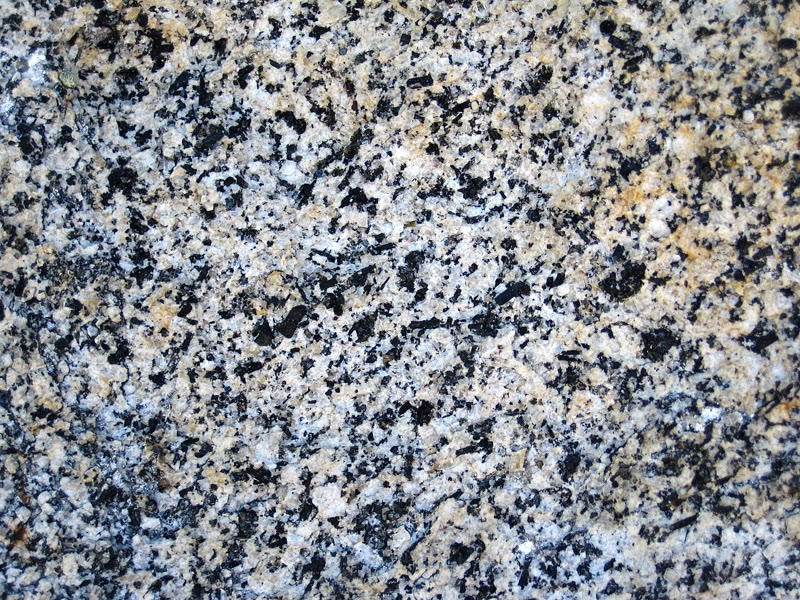
\includegraphics[height=4.4cm]{images/book2/g12-stjohn-granodiorite.jpg}

{\small À esquerda: \omterm{def:g11:igneous-rocks:rock-names}{andesito}, uma \omterm{def:g11:igneous-rocks:volcanic-plutonic}{rocha vulcânica} de grãos finos dos arcos.
À direita: \omterm{def:g12:subduction-magmatism:granodiorite}{granodiorito} da Sierra Nevada, com plagioclásio branco, quartzo
cinzento e biotita e hornblenda pretas. Fotografias James St.~John
(CC~BY~2.0).}
\end{omfigure}
% ledger: photo:g12-andesite, photo:g12-granodiorite

Em média, a \omterm{def:g12:continental-crust:continental-crust}{crosta continental} superior contém cerca de \qty{67}{\percent}
de \ce{SiO2}: ela é \omterm{def:g11:igneous-rocks:felsic-mafic}{félsica}, como os granitos que os arcos produzem em
quantidade nos seus \omterm{def:g12:subduction-magmatism:batholith}{batólitos}.
% ledger: rg14:crust (upper crust SiO2 66.6 wt %), tulane:magma-types, tulane:intrusions

\begin{definition}[Batólito]\label{def:g12:subduction-magmatism:batholith}
Um \emph{batólito}\index{batolito@batólito} é uma grande massa de \omterm{def:g11:igneous-rocks:volcanic-plutonic}{rocha plutônica} que cobre
mais de \qty{100}{km^2} onde a erosão a expôs. Ele se forma onde muitos
\omterm{def:g11:igneous-rocks:intrusion}{plútons}, intrudidos uns depois dos outros, se juntam sob a superfície.
\end{definition}
% ledger: earle:batholith, tulane:intrusions

Um dos maiores do mundo, o Complexo Plutônico da Costa, se estende ao longo
da costa do Pacífico, da região de Vancouver, no oeste do Canadá, até o
sudeste do Alasca. O \omterm{def:g12:subduction-magmatism:batholith}{batólito} da Sierra Nevada, na Califórnia, se formou
acima de uma \omterm{def:g11:subduction-zones:subduction}{zona de subducção}; a maioria dos seus granitos de Yosemite se
cristalizou no Cretáceo, entre 105 e 85 milhões de anos atrás. As rochas
acima deles foram desgastadas ao longo de milhões de anos, e os \omterm{def:g11:igneous-rocks:intrusion}{plútons} que
esfriaram em profundidade hoje formam as montanhas.
% ledger: earle:batholith, nps:yosemite, photo:g12-sierra-nevada (St. John description), ics:base.Cretaceous

\begin{omfigure}
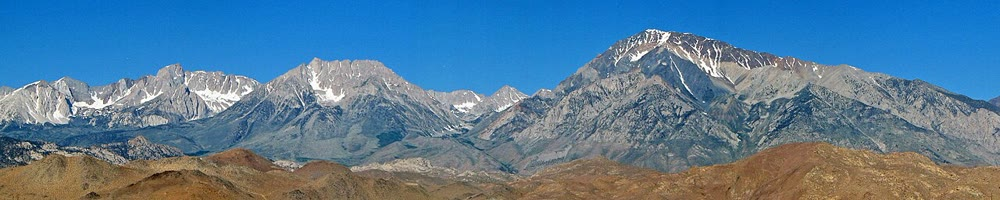
\includegraphics[width=0.94\linewidth]{images/book2/g12-stjohn-sierra-nevada-batholith.jpg}

{\small A Sierra Nevada, vista do leste: granito e \omterm{def:g12:subduction-magmatism:granodiorite}{granodiorito} do \omterm{def:g12:subduction-magmatism:batholith}{batólito}
da Sierra Nevada, que se cristalizaram em profundidade acima de uma \omterm{def:g11:subduction-zones:subduction}{zona de
subducção} no Cretáceo. Fotografia James St.~John (CC~BY~2.0).}
\end{omfigure}
% ledger: photo:g12-sierra-nevada, nps:yosemite

\section{Como os continentes crescem}

\begin{definition}[Crescimento continental]\label{def:g12:subduction-magmatism:continental-growth}
O \emph{crescimento continental}\index{crescimento continental} é a adição
de nova \omterm{def:g12:continental-crust:continental-crust}{crosta continental}, formada a partir do manto, principalmente pelo
magmatismo dos arcos. O crescimento líquido dos continentes é essa adição
menos a \omterm{def:g12:continental-crust:continental-crust}{crosta continental} que volta ao manto.
\end{definition}
% ledger: sv09:growth, ss09:balance

Os arcos são onde se forma a rocha leve dos continentes. As estimativas do
magma que os arcos acrescentam hoje são de cerca de \qty{1.5}{km^3} por ano
nos arcos insulares e \qty{1.0}{km^3} por ano nos arcos continentais; em
média no longo prazo, cerca de \qty{2.7}{km^3} por ano. Mas as \omterm{def:g11:subduction-zones:subduction}{zonas de
subducção} também levam \omterm{def:g12:continental-crust:continental-crust}{crosta continental} de volta ao manto: sedimentos
arrastados com a \omterm{def:g11:subduction-zones:slab}{laje} e pedaços da placa que se sobrepõe raspados por baixo,
cerca de \qty{3.2}{km^3} por ano. Os dois números são próximos, e o
crescimento líquido dos continentes nas últimas centenas de milhões de anos
pode ter sido nulo, ou até negativo.
% ledger: sv09:growth, ss09:balance

Os continentes também crescem pelas bordas de outra maneira. A \omterm{def:g12:continental-crust:continental-crust}{crosta
continental} é leve demais para ser subductada, por isso, quando uma placa
leva um continente a uma fossa, os dois continentes são soldados numa
colisão (\cref{ch:g12:mountain-building}). Cada continente tem um núcleo
antigo, um \omterm{def:g12:continental-crust:craton}{cráton}, cercado por cinturões de rochas mais jovens, as \omterm{def:g12:continental-crust:root}{raízes}
deformadas de antigos cinturões de montanhas, acrescentados uns depois dos
outros às suas bordas (\cref{ch:g12:continental-crust}).
% ledger: tulane:no-subduct (continental crust too buoyant to subduct), earle:collision, tulane:cratons

\section{Exercícios}

\begin{exercise}[$\star$]\label{exo:g12:subduction-magmatism:1}
Dê a palavra: (a) uma fileira de vulcões paralela a uma fossa, na placa que
não afunda; (b) a fusão causada pela adição de água a uma rocha; (c) uma
\omterm{def:g11:igneous-rocks:volcanic-plutonic}{rocha plutônica} com mais plagioclásio que feldspato potássico e mais de
\qty{20}{\percent} de quartzo; (d) uma massa de \omterm{def:g11:igneous-rocks:volcanic-plutonic}{rocha plutônica} maior que
\qty{100}{km^2}; (e) a adição de nova \omterm{def:g12:continental-crust:continental-crust}{crosta continental} formada a partir do
manto.
\end{exercise}

\begin{exercise}[$\star$]\label{exo:g12:subduction-magmatism:2}
Em 18 de maio de 1980, a coluna de cinzas do monte Santa Helena subiu a mais
de \qty{24}{km} em menos de 15 minutos. (1) Qual foi a sua menor velocidade
média de subida, em \unit{km/h} e em \unit{m/s}? (2) Compare-a com a
velocidade da explosão lateral, de pelo menos \qty{480}{km/h}.
\end{exercise}

\begin{exercise}[$\star$]\label{exo:g12:subduction-magmatism:3}
Dos 1214 vulcões do catálogo ativos desde o fim da última era glacial, 838
ficam acima de uma \omterm{def:g11:subduction-zones:subduction}{zona de subducção}. (1) Que porcentagem é essa? (2) De que
lado de uma fossa ficam esses vulcões? (3) Por que não há nenhum entre a
fossa e a frente vulcânica?
\end{exercise}

\begin{exercise}[$\star$]\label{exo:g12:subduction-magmatism:4}
Uma rocha de grãos grossos contém \qty{25}{\percent} de quartzo,
\qty{45}{\percent} de plagioclásio, \qty{15}{\percent} de feldspato
potássico e \qty{15}{\percent} de biotita e hornblenda. (1) Que fração do
seu feldspato é plagioclásio? (2) É um \omterm{def:g12:subduction-magmatism:granodiorite}{granodiorito}?
\end{exercise}

\begin{exercise}[$\star$]\label{exo:g12:subduction-magmatism:5}
Dê duas razões pelas quais os vulcões dos arcos têm erupções mais
explosivas que os das dorsais.
\end{exercise}

\begin{exercise}[$\star\star$]\label{exo:g12:subduction-magmatism:6}
(1) Uma frente vulcânica fica a \qty{150}{km} da sua fossa, acima de uma
\omterm{def:g11:subduction-zones:slab}{laje} que mergulha \ang{35}. A que profundidade fica a \omterm{def:g11:subduction-zones:slab}{laje} sob ela?
(2) Compare com a média de \qty{105}{km}.
\end{exercise}

\begin{exercise}[$\star\star$]\label{exo:g12:subduction-magmatism:7}
Suponha que a \omterm{def:g11:subduction-zones:slab}{laje} fica a \qty{105}{km} sob todas as frentes vulcânicas. A
que distância da fossa fica a frente quando a \omterm{def:g11:subduction-zones:slab}{laje} mergulha \ang{20}, e
quando mergulha \ang{45}? O que isso diz sobre onde procurar o arco?
\end{exercise}

\begin{exercise}[$\star\star$]\label{exo:g12:subduction-magmatism:8}
A \qty{100}{km}, a pressão é de cerca de \qty{3.16}{GPa}. (1) Usando $T =
-5.104P^2 + 132.9P + 1120.7$ ($P$ em \unit{GPa}, $T$ em \unit{\celsius}),
calcule a temperatura em que o \omterm{def:g11:ocean-ridges:peridotite}{peridotito} seco começa a se fundir ali.
(2) Com água, ele começa a se fundir a cerca de \qty{1000}{\celsius}. Em
quanto a água a abaixa? (3) A cunha do manto ali está a, digamos,
\qty{1300}{\celsius}. Ela se funde seca? Molhada?
\end{exercise}

\begin{exercise}[$\star\star$]\label{exo:g12:subduction-magmatism:9}
A avalanche de detritos do monte Santa Helena deslocou cerca de
\qty{2.5}{km^3} de rocha. Os arcos acrescentam cerca de \qty{2.7}{km^3} de
nova crosta por ano. (1) Quantos dias do magmatismo de arco do mundo a
avalanche representa? (2) Por que a comparação é só uma questão de
tamanho?
\end{exercise}

\begin{exercise}[$\star\star$]\label{exo:g12:subduction-magmatism:10}
(1) Quanta crosta nova os arcos acrescentam em um milhão de anos a
\qty{2.7}{km^3} por ano? (2) A \omterm{def:g12:continental-crust:continental-crust}{crosta continental} contém cerca de
\qty{9e9}{km^3}. Quanto tempo os arcos sozinhos levariam para produzir esse
volume, se nada dele se perdesse? (3) Compare com a idade da Terra, 4.5
bilhões de anos.
\end{exercise}

\begin{exercise}[$\star\star$]\label{exo:g12:subduction-magmatism:11}
(1) No corte através do Japão, por que muitos terremotos com menos de
\qty{70}{km} de profundidade são deixados de fora quando se ajusta a \omterm{def:g11:subduction-zones:slab}{laje}?
(2) Os terremotos profundos ficam a \qty{116}{km} de profundidade a
\ang{140.5}~Leste e a \qty{80}{km} a \ang{141.5}~Leste, com \qty{86.4}{km}
por grau. Calcule o mergulho da \omterm{def:g11:subduction-zones:slab}{laje}.
\end{exercise}

\begin{exercise}[$\star\star\star$]\label{exo:g12:subduction-magmatism:12}
Mostre que, para uma frente a uma distância $d$ da fossa acima de uma \omterm{def:g11:subduction-zones:slab}{laje}
de mergulho $\theta$, a distância medida ao longo da \omterm{def:g11:subduction-zones:slab}{laje}, da fossa até o
ponto sob a frente, é $d/\cos\theta$. Para o Japão ($d = \qty{270}{km}$,
$\theta = \ang{20}$), quanto ela mede? A placa do Pacífico se move em
direção ao Japão a cerca de \qty{83}{mm} por ano; tomando essa velocidade
ao longo de toda a \omterm{def:g11:subduction-zones:slab}{laje}, quanto tempo um pedaço de fundo do mar leva para ir
da fossa até sob os vulcões?
\end{exercise}
% ledger: usgs:tohoku (83 mm/yr)

\begin{exercise}[$\star\star\star$]\label{exo:g12:subduction-magmatism:13}
A câmara magmática do monte Santa Helena tem cerca de \qty{1}{km} de
largura e se estende de cerca de 6 a \qty{14}{km} de profundidade.
(1) Tratando-a como um cilindro vertical, estime o seu volume. (2) Compare-o
com os \qty{2.5}{km^3} da avalanche. (3) Calcule a \omterm{def:g12:metamorphic-rocks:lithostatic}{pressão litostática} no
seu topo e na sua base ($\rho =
\qty{2830}{kg/m^3}$, $g = \qty{9.81}{m/s^2}$).
\end{exercise}

\begin{exercise}[$\star\star\star$]\label{exo:g12:subduction-magmatism:14}
Os arcos acrescentam cerca de \qty{2.7}{km^3} de crosta por ano, e as \omterm{def:g11:subduction-zones:subduction}{zonas
de subducção} levam de volta cerca de \qty{3.2}{km^3}. (1) Qual é a variação
líquida por milhão de anos? (2) Em 500 milhões de anos, que fração de uma
crosta de \qty{9e9}{km^3} é isso? (3) Os autores dizem que o crescimento
líquido é ``efetivamente nulo''. Por quê, dada a incerteza de cada
estimativa?
\end{exercise}

\begin{exercise}[$\star\star\star$]\label{exo:g12:subduction-magmatism:15}
Um \omterm{def:g12:subduction-magmatism:batholith}{batólito} expõe \qty{20000}{km^2} de \omterm{def:g12:subduction-magmatism:granodiorite}{granodiorito} cujos \omterm{def:g11:igneous-rocks:intrusion}{plútons} se
solidificaram entre 5 e \qty{15}{km} de profundidade. (1) Estime o volume
de magma que ele representa, tomando-o com \qty{10}{km} de espessura.
(2) A \qty{1}{km^3} por ano, a taxa de todos os arcos continentais do mundo
juntos, quanto tempo eles levariam para produzi-lo? O que isso diz sobre o
tempo durante o qual um \omterm{def:g12:subduction-magmatism:batholith}{batólito} é construído?
(3) Quanta rocha precisou ser erodida de cima dele antes que ele pudesse ser
visto?
\end{exercise}

\begin{problem}[{Problema de fim de semana --- sob os vulcões do Japão}]
\label{pb:g12:subduction-magmatism:1}
% ledger: data:b2-usgs-ne-japan, data:gvp, data:pb2002, sa06:slab-depth, hirschmann:solidus, wang20:wet-solidus, earle:arc-water, data:prem
% values (arc_magmatism.py): Megata 139.725, Iwate 141.001, trench 144.12; bins 140.5/141/141.5: 116.4/98.15/80.35 km; P_100km 3.157, dry_T_100km 1489
Os vulcões do nordeste do Japão entre \ang{37.5} e \ang{40.5}~Norte ficam
entre \ang{139.7}~Leste (Megata, o mais a oeste) e \ang{141.0}~Leste (Iwate,
o mais a leste); a Fossa do Japão fica a \ang{144.1}~Leste. A tabela dá a
profundidade mediana dos terremotos com mais de \qty{70}{km} de
profundidade em três faixas de longitude, 1976--2025. Tome \qty{111.2}{km}
para um grau de latitude.

\begin{center}
\small
\begin{tabular}{|l|c|c|c|}
\hline
longitude (\unit{\degree}~L) & 140.5 & 141.0 & 141.5 \\ \hline
profundidade mediana (\unit{km}) & 116 & 98 & 80 \\ \hline
\end{tabular}
\end{center}

\medskip
\noindent\textbf{Parte I --- A frente vulcânica.}
\begin{enumerate}
  \item Mostre que um grau de longitude a \ang{39}~Norte vale cerca de
        \qty{86.4}{km}.
  \item A que distância da fossa fica a frente vulcânica?
  \item Qual é a largura do arco, de Iwate a Megata?
  \item Em que placa ficam os vulcões, e de que lado da fossa?
  \item Por que não há vulcões entre a fossa e Iwate?
\end{enumerate}

\medskip
\noindent\textbf{Parte II --- O corte dos terremotos.}
\begin{enumerate}[resume]
  \item Em quantos quilômetros as profundidades medianas mudam de
        \ang{140.5} a \ang{141.5}~Leste?
  \item Ao longo de que distância horizontal?
  \item Calcule o mergulho da \omterm{def:g11:subduction-zones:slab}{laje}.
  \item Prolongue a reta a partir de \ang{141.0}~Leste, \qty{98}{km}, até a
        superfície. Onde ela a atinge, e a que distância isso fica da fossa?
  \item Sugira por que a \omterm{def:g11:subduction-zones:slab}{laje} é menos íngreme perto da fossa do que mais
        abaixo.
\end{enumerate}

\medskip
\noindent\textbf{Parte III --- A laje sob os vulcões.}
\begin{enumerate}[resume]
  \item Calcule $H = d\tan\theta$ com a distância da questão 2 e um mergulho
        de \ang{20}.
  \item Compare-a com a profundidade mediana sob a frente.
  \item Compare ambas com a faixa mundial, de 72 a \qty{173}{km}, e com a
        média, \qty{105}{km}.
  \item A que profundidade fica a \omterm{def:g11:subduction-zones:slab}{laje} sob Megata, usando a reta da
        questão 9?
  \item Tomando a crosta do arco com cerca de \qty{35}{km} de espessura, o
        topo da \omterm{def:g11:subduction-zones:slab}{laje} sob a frente fica na crosta ou no manto? A que
        distância abaixo da base da crosta ele fica?
\end{enumerate}

\medskip
\noindent\textbf{Parte IV --- De onde vem a água.}
\begin{enumerate}[resume]
  \item Onde a água da \omterm{def:g11:subduction-zones:slab}{laje} entrou nas suas rochas, e em que mineral grande
        parte dela fica retida?
  \item A \qty{100}{km}, a pressão é de cerca de \qty{3.16}{GPa}. Calcule o
        solidus seco ali com $T = -5.104P^2 + 132.9P + 1120.7$.
  \item Com água, o solidus fica entre 950 e \qty{1000}{\celsius}. Em quanto
        a água o abaixa?
  \item Por que a própria \omterm{def:g11:subduction-zones:slab}{laje} fria não pode ser a fonte do magma?
  \item Resuma: a que profundidade fica a \omterm{def:g11:subduction-zones:slab}{laje} sob a frente vulcânica do
        nordeste do Japão?
\end{enumerate}
\end{problem}
